\documentclass[aspectratio=169, 14pt]{beamer}
\usepackage[utf8]{inputenc}
\usepackage{amsmath}
\usepackage{xeCJK}
\usepackage{tipa}
\usepackage{graphicx}
\usepackage[ruled, lined, linesnumbered, commentsnumbered]{algorithm2e}
\usepackage[edges]{forest}
\usepackage{tikz}
\usetikzlibrary{arrows}
\usetikzlibrary {arrows.meta}
\usetikzlibrary{calc,shadows.blur,fit,positioning}
\usetikzlibrary{matrix,backgrounds}
\usepackage{minted}
\usepackage{fontawesome5}
\usepackage{booktabs}
\usepackage{caption}
\usepackage{hyperref}
\hypersetup{
    colorlinks=true,
    linkcolor=blue,
    filecolor=magenta,      
    urlcolor=cyan,
    }
\urlstyle{same}
\usetheme{metropolis}
\metroset{block=fill}
\usecolortheme{default}
\definecolor{darkmidnightblue}{rgb}{0.0, 0.2, 0.4}
\definecolor{LightGray}{gray}{0.9}


%------------------------------------------------------------
%This block of code defines the information to appear in the
%Title page
\title[Database Principles and Applications] %optional
{数据库原理与应用}

\subtitle{Introduction to Database}

\author[CHEN Zhongpu] % (optional)
{CHEN Zhongpu}

\institute[] % (optional)
{
  School of Computing and Artificial Intelligence \\
  \href{mailto:zpchen@swufe.edu.cn}{zpchen@swufe.edu.cn}
}

\date[] % (optional)
{SWUFE, Fall 2022}

%End of title page configuration block
%------------------------------------------------------------


%------------------------------------------------------------
%The next block of commands puts the table of contents at the 
%beginning of each section and highlights the current section:

% \AtBeginSection[]
% {
%   \begin{frame}
%     \frametitle{Table of Contents}
%     \tableofcontents[currentsection]
%   \end{frame}
% }
%------------------------------------------------------------


\begin{document}

%The next statement creates the title page.
\frame{\titlepage}

%---------------------------------------------------------
%This block of code is for the table of contents after
%the title page
% \begin{frame}
% \frametitle{Table of Contents}
% \tableofcontents
% \end{frame}
%--------------------------------------------------------
\begin{frame}
\frametitle{思考}
\begin{columns}
    \column{0.5\textwidth}
    \includegraphics[width=.9\textwidth]{image/tencent}
    \column{0.5\textwidth} 
    腾讯公司的什么资产最值钱?
\end{columns}
\end{frame}

\begin{frame}
    \begin{center}
        \textcolor{red}{\large 中共中央关于坚持和完善中国特色社会主义制度}

        \textcolor{red}{推进国家治理体系和治理能力现代化若干重大问题的决定}
    \end{center}
    \begin{quote}
        `` 健全劳动、资本、土地、知识、技术、管理和\alert{数据}等生产要素按贡献参与分配的机制。"
    \end{quote}
\pause
    \begin{center}
        \includegraphics[width=.5\textwidth]{image/rmb}
    \end{center}

\end{frame}

{
    % \usebackgroundtemplate{\transparent{0.3}{\begin{picture}
    %     \includegraphics[height=0.7\paperheight]{cover}
    % \end{picture}    
    % }}
\usebackgroundtemplate{
  \tikz[overlay,remember picture] 
  \node[opacity=0.3, at=(current page.south east),anchor=south east, yshift=2cm,xshift=4cm] {
    \includegraphics[height=0.6\paperheight]{cover}};
}
    \begin{frame}
        \section{\textcolor{darkmidnightblue}{1. 什么是数据库?}}

        Data\alert{base}

        \pause

        \begin{quote}
            the main place where a person lives and works, or a place that a company does business from (基地;总部)
            \begin{flushright}
                --- Cambridge dictionary
            \end{flushright}
        \end{quote}
        \begin{itemize}
            \item I spend a lot of time in Brussels, but London is still my base. 我经常呆在布鲁塞尔,但伦敦仍然是我的基地。
        \end{itemize}
    \end{frame}

}


\begin{frame}
    \frametitle{数据库}
\begin{block}{百度}
    是一个长期存储在计算机内的、有组织的、可共享的、统一管理的大量数据的集合。
\end{block}
\begin{block}{Wikipedia}
    A database is an organized collection of data stored and accessed electronically from a computer system.
\end{block}
\end{frame}

\begin{frame}
    \frametitle{数据库}
    \includegraphics[width=0.5\paperwidth]{image/oracle}
    \begin{exampleblock}{Oracle}
        是结构化信息或数据(一般以电子形式存储在计算机系统中)的有组织的集合,通常由数据库管理系统 (DBMS) 来控制。

        在现实中,数据、DBMS 及关联应用一起被称为\alert{数据库系统},通常简称为数据库。 
    \end{exampleblock}
\end{frame}

\begin{frame}
    \frametitle{数据库系统}
    \begin{block}{课本}
        A database-management system (DBMS) is a collection of interrelated data and a set of programs to access those data.
    \end{block}
    并且,数据库系统有两大基本需求:\alert{convenient} 和 \alert{efficient}。
\end{frame}

\begin{frame}
    \frametitle{国产数据库系统}
    \begin{columns}
        \column{0.6\textwidth}<1->
        \begin{table}
            \caption{DB Rank}
            \begin{tabular}{lll}
              \toprule
              Rank & DBMS & Database Model \\
              \midrule
              1 & \textcolor{blue}{Oracle} & Relational \\
              2 & \textcolor{blue}{MySQL} & Relational \\
              3 & \textcolor{blue}{SQL Server} & Relational \\
              4 & \textcolor{blue}{PostgreSQL} & Relational \\
              5 & \textcolor{blue}{MongoDB} & Document \\
              6 & \textcolor{blue}{Redis} & Key value \\
              \bottomrule
            \end{tabular}
        \end{table}
        \column{0.4\textwidth}<2->
        \begin{itemize}
            \item OceanBase (阿里)
            \item TiDB (PingCAP)
            \item ...
        \end{itemize}
    \end{columns}

\end{frame}

\begin{frame}
\section{\textcolor{darkmidnightblue}{2. 数据库应用}}
    
在互联网时代,你几乎找不到不使用数据库的场合。
\end{frame}

\begin{frame}
    \frametitle{电子商务}
    \begin{center}
        \includegraphics[width=.55\paperwidth]{image/dict}
    \end{center}

    \begin{itemize}
        \item 销售:客户,产品,购买信息
        \item 记账:支付,收据,余额
        \item 物流
        \item ...
    \end{itemize}
\end{frame}

\begin{frame}
    \frametitle{企业机构}
    
    \includegraphics[width=.55\paperwidth]{image/swufe}
    \begin{itemize}
        \item 学生
        \item 教师
        \item 课程、选课
        \item ...
    \end{itemize}

    \begin{tikzpicture}
        \node[fill=yellow,blur shadow={shadow xshift=-0.5ex},
        text width=20em,anchor=south west,rounded corners]
        {课程将以「大学」为背景介绍数据库};
    \end{tikzpicture}

\end{frame}

\begin{frame}
    \begin{itemize}
        \item \faIcon{youtube} 视频信息、播放次数
        \item \faIcon{twitter} 发帖、评论、点赞
        \item \faIcon{plane} 航班、座位、票务
        \item ...
    \end{itemize} 
    \pause
即使某些单机应用,也可能使用 \href{https://www.sqlite.org/famous.html}{SQLite} 数据库(包括iOS、Android等)。

\includegraphics[width=.3\paperwidth]{image/sqlite}

\end{frame}

\begin{frame}
    \frametitle{数据库应用}
    数据库的应用大致可以分为两类:
    \begin{itemize}
        \item 在线交易/联机事务处理 (online transaction processing)
        \item 数据分析 (data analytics)
    \end{itemize}   
\includegraphics[width=.5\textwidth]
{image/beer}

\end{frame}

\begin{frame}
    \section{\textcolor{darkmidnightblue}{3. 数据库系统的作用}}
    如果没有数据库系统,那么人们应该如何管理数据?
\end{frame}

\begin{frame}[fragile]
\begin{quote}
    \begin{columns}
        \column{0.5\textwidth} 
        记得早先少年时,\\
        大家诚诚恳恳,\\
        说一句,是一句。\\
        \bigskip
        清早上火车站,\\
        长街黑暗无行人,\\
        卖豆浆的小店冒着热气。\\
        \column{0.5\textwidth}
        从前的日色变得慢,\\
\alert{车,马,邮件都慢},\\
一生只够爱一个人。\\
\bigskip
从前的锁也好看,\\
钥匙精美有样子。\\
你锁了,人家就懂了。\\
    \end{columns}
\end{quote}
\end{frame}

\begin{frame}
    \frametitle{如果没有 DBMS}

    \begin{columns}
        \column{0.4\textwidth}
        {\Large \faIcon[regular]{pen}} \faIcon[regular]{plus} {\huge \faIcon[regular]{sticky-note}}

        (非电子化的)纸和笔

        \column{0.5\textwidth}
        {\LARGE \faIcon[regular]{file} \faIcon[regular]{folder} \faIcon[regular]{file-archive} \faIcon[regular]{file-word} \faIcon[regular]{file-excel} \faIcon[regular]{file-powerpoint} \faIcon[regular]{file-pdf}} 

        操作系统的文件
    \end{columns}
\end{frame}
\begin{frame}
    考虑一个简单的\alert{教务信息管理系统},并假设数据全部都保存在普通 TXT 文件里面。该系统支持下列功能:
\begin{itemize}
    \item 添加新的学生、老师、课程
    \item 学生选课
    \item 给学生打分
    \item 计算GPA
\end{itemize}
\end{frame}

\begin{frame}[fragile]

    \begin{columns}
        \column{0.2\textwidth}
        {\large \textcolor{blue}{\texttt{instructor.txt}}}
        \column{0.7\textwidth} 
        \begin{verbatim}
            name|department|salary
            Bob|Computer Science|1000
            Alice|Foreign Language|2000        
         \end{verbatim}
    \end{columns}
\pause
    \begin{minted}[bgcolor=LightGray, fontsize=\footnotesize]{java}
private void addInstructor(String name, String depart, double salary)    
        throw IOException {
    String path = "/home/zhongpu/instructor.txt";
    String s = "%s|%s|%f";
    Files.writeString(Path.of(path),
        String.format(s, name, depart, salary) + System.lineSeparator(),
        StandOperation.CREATE, StandOperation.APPEND); 
}
    \end{minted}
  
\end{frame}

\begin{frame}
    \frametitle{文件处理系统}

    \begin{block}{File-processing system}
        将记录存储在不同的文件,并需要不同的应用程序来处理文件。        
    \end{block}
    显然,用文件处理系统管理上述信息有很多的缺点。
\end{frame}

\begin{frame}[fragile]

    \begin{columns}
        \column{0.2\textwidth}
        {\large \textcolor{blue}{\texttt{instructor}}}
        \column{0.7\textwidth} 

\begin{table}
    \begin{tabular}{lll}
      \toprule
      name & department & salary \\
      \midrule
      Bob & Computer Science & 1000 \\
      Alice & Foreign Language & 2000 \\
      \bottomrule
    \end{tabular}
\end{table}
    \end{columns}
\begin{minted}[bgcolor=LightGray, fontsize=\footnotesize]{sql}
INSERT INTO instructor
VALUES ('Bob', 'Computer Science', 1000);
\end{minted}
\end{frame}

\begin{frame}
    \frametitle{文件处理系统(缺点)}

\begin{itemize}
    \item \alert{数据冗余和不一致} (data redundancy and inconsistency)
\end{itemize}

\begin{columns}
    \column{0.5\textwidth}

    \faIcon{graduation-cap} \(
      \begin{cases}
        Computer\ Degree \\
        Management\ Degree 
      \end{cases}
      \)
    \column{0.5\textwidth}
    \begin{tikzpicture}
        \node[fill=yellow,blur shadow={shadow xshift=-0.5ex},
        text width=14em,anchor=south west,rounded corners]
        {数据冗余意味着更高的存储代价,并且相同数据的多个副本可能会导致数据不一致的情况。};
    \end{tikzpicture}
\end{columns}
\pause
\begin{itemize}
    \item \alert{数据隔离
    } (data isolation)
\end{itemize}

\begin{tikzpicture}
    \node[fill=yellow,blur shadow={shadow xshift=-0.5ex},
    text width=25em,anchor=south west,rounded corners]
    {数据分散在不同的文件,也可能使用不同的格式。
    因此,写新的程序获取数据很困难。
    };
\end{tikzpicture}

\end{frame}

\begin{frame}
\begin{itemize}
    \item \alert{访问数据困难
    } (difficulty in accessing data)
\end{itemize}
    \begin{block}{新需求}
假设需要获取每个省份的学生列表,而目前程序中只有返回所有学生列表的功能。
    \end{block}

    \begin{table}
        \begin{tabular}{lll}
          \toprule
          name & department & province \\
          \midrule
          Jack & Computer Science & Shanghai \\
          \bottomrule
        \end{tabular}
    \end{table}

\end{frame}

\begin{frame}
    \begin{itemize}
        \item \alert{完整性问题
        } (integrity problem)
    \end{itemize}

    \begin{table}
        \begin{tabular}{lll}
          \toprule
          name & department & salary \\
          \midrule
          Bob & Computer Science & 1000 \\
          \bottomrule
        \end{tabular}
    \end{table}
    某些值可能要满足一定约束 (constraint)。比如 salary > 0。

    尽管这可能通过程序中添加代码实现约束,但灵活性不够。比如可能会添加新的约束。
\end{frame}

\begin{frame}
    \begin{itemize}
        \item \alert{安全性问题
        } (security problem)
    \end{itemize}
    \begin{table}
        \begin{tabular}{lll}
          \toprule
          name & department & \textcolor{red}{salary} \\
          \midrule
          Bob & Computer Science & \textcolor{red}{1000} \\
          \bottomrule
        \end{tabular}
    \end{table}

    \emph{不是所有的用户都能访问所有的数据}。比如教务人员只能查到老师的姓名、学院等信息,不应该看到工资信息。

    在文件处理系统上实现安全约束也比较困难。    
\end{frame}

\begin{frame}
    \begin{center}
        \includegraphics[height=.4\paperheight]{image/money}
    \end{center}
    \begin{itemize}
        \item \alert{并发访问异常
        } (concurrent-access anomalies)

        假设你的账户有10万元,同一时刻有两笔支出(分别1万和2万),那么最后的结果可能是不正确的(9万或8万)。
        \item \alert{原子性问题} (atomicity problems)
        
        你在付款的过程中,系统出现崩溃,此时可能会出现你的钱被扣除,但对象没有收到的情况。
    \end{itemize}

\end{frame}

\begin{frame}
    \frametitle{}

    \begin{quote}
        上述的(以及其他的)缺点,推动了 1960 和 1970 年代数据库系统的发展,并促使了从\alert{文件处理系统}到\alert{数据库系统}的转变。
    \end{quote}

    \begin{center}
        {\Huge \faIcon{file} \faIcon{arrow-right} \faIcon{database}}
    \end{center}

\end{frame}

\begin{frame}
    \section{\textcolor{darkmidnightblue}{4. 数据视图}} 
    数据库系统的一个重要作用就是为用户提供了一个\alert{抽象的数据视图} (abstract view of data)。

    \pause
    \begin{block}{view}
        an opinion, belief, or idea, or a way of thinking about something (观点;见解;看法)
    \end{block}
\end{frame}
\begin{frame}
    \frametitle{什么是抽象}    
抽象(abstraction)是计算机中最重要的概念之一;其主要好处就在于它使你能忽略无关的细节。

\includegraphics[width=.45\textwidth]{image/house.png}
\includegraphics[width=.45\textwidth]{image/home.png}
\end{frame}

\begin{frame}
    \frametitle{数据抽象}  
    
    \begin{columns}
        \column{0.475\textwidth}<1->
        \begin{tikzpicture}[
            node distance=2cm,
            title/.style={font=\color{black!50}\ttfamily, fill=orange!30,},
            typetag/.style={rectangle, draw=black!50, font=\ttfamily, anchor=west}
          ]
            \node (decomp) [title] { \normalsize 视图层 (view level)};
          
            \node (di) [below=of decomp.west, typetag, yshift=0.5cm] { view 1 };
            \node (dr) [right=of di.west, typetag] { view 2 };
            \node (dots) [right=of dr.west] {...};
            \node (dnc) [right=of dots.west, typetag, xshift=-1cm] { view n };
          
            \node [draw=black!50,  fit={(decomp) (di) (dr) (dots) (dnc)}] (view){};
    
            \node[draw=black!50, below=of view, yshift=1cm,title](logical){逻辑层 (logical level)};
    
            \node[draw=black!50, below=of logical, yshift=1cm,title](physical){物理层 (physical level)}; 
    
            \draw[-, thick] (view) -- (logical);
            \draw[-, thick] (logical) -- (physical);
    
          \end{tikzpicture}
          \column{0.475\textwidth}<2->
          \begin{itemize}
            \item 物理层:数据如何存储
            \item 逻辑层:存储什么数据,及数据之间的关系
          \end{itemize}

          \begin{tikzpicture}
            \node[fill=yellow,blur shadow={shadow xshift=-0.5ex},
            text width=15em,anchor=south west,rounded corners]
            {物理数据的独立性(physical data independence)
            };
        \end{tikzpicture} 
    \end{columns}
\end{frame}

\begin{frame}
\begin{center}
    Developers hide the complexity from users.
    \includegraphics[height=.8\paperheight]{image/heart}
\end{center}
    

\end{frame}

\begin{frame}
    \frametitle{数据模型}
    \begin{block}{数据模型}
        数据模型 (data model) 描述数据、数据关系、数据语义和一致性约束的概念化工具的集合。
    \end{block}

    \begin{columns}
        \column{0.6\textwidth}
        \begin{quote}
            A database model is a type of data model that determines the logical structure of a database.
        \end{quote}
        \column{0.4\textwidth}
        \begin{enumerate}
            \item 关系模型
            \item 实体-联系模型
            \item 半结构化数据模型
            \item 基于对象的数据模型
        \end{enumerate} 
    \end{columns}

\end{frame}
\begin{frame}[fragile]
    \begin{itemize}
        \item 关系模型 (relational model):表 (table)就是关系 (relation)。\alert{是最常用的数据模型}。
    \end{itemize}


    \begin{columns}
        \column{0.7\textwidth}<1->
        \begin{tikzpicture}[head/.style={fill=blue!30}, >=Stealth]
            \matrix (mat) [matrix of nodes, row sep=-\pgflinewidth, nodes=draw, nodes={minimum width=2.8cm, minimum height=1cm, anchor=center}]
            {
            \node[head](name){name}; & \node[head](department) {department}; & \node[head](salary){salary}; \\
            \node{Bob}; & \node{Comp. Sci.}; & \node(1000){1000}; \\
            \node{Wu}; & \node{Finance}; & \node(1200){1200}; \\
            };
            \node[above=of department,yshift=-0.5cm](column){\alert{列 (column)}};
            \draw[->, thick, red] (department) -- (column);
            \draw[->, thick, red] (salary) -- (column);
            \draw[->, thick, red] (name) -- (column);
            
            \node[right=of 1000, xshift=-0.5cm, yshift=-0.5cm](row){\alert{行 (row)}};
            \draw[->, thick, red] (1000) -- (row);
            \draw[->, thick, red] (1200) -- (row);
            \end{tikzpicture}
            \column{0.28\textwidth}<2->
            \begin{figure}
                \includegraphics[width=.8\textwidth]{image/codd}
                \caption*{Edgar F. Codd (Turing Award 1981)}
              \end{figure}
    \end{columns}
\end{frame}

\begin{frame}

\includegraphics[width=.475\textwidth]{table/instructor}    
\includegraphics[width=.475\textwidth]{table/department} 
\end{frame}

\begin{frame}[fragile]
\begin{itemize}
    \item<1-> 实体-联系模型 (entity-relationship model): the (E-R) data model uses a collection of basic objects, called \textbf{entities}, and \textbf{relationships} among these objects. \alert{广泛应用于数据库设计}。
    \item<2-> 半结构化数据模型 (semi-structured data model): individual data items of the same type may have different sets of attributes. \alert{广泛应用于互联网和大数据场景}。 
    \begin{minted}{json}
{
    "employees":[
        {"firstName":"John", "lastName":"Doe"},
        {"firstName":"Anna", "lastName":"Smith"}
    ]
}                    
    \end{minted}
\end{itemize}
\end{frame}

\begin{frame}[fragile]
\begin{itemize}
    \item 基于对象的数据模型 (object-based data model)
\end{itemize}

\begin{columns}
    \column{0.1\textwidth}
    {\Huge \faIcon{dog}}
    \column{0.85\textwidth} 
    \begin{minted}{java}
class Dog {
    private String name;
    private int age;
    public void eat() {
        // ...
    }
    // ...
}
    \end{minted} 
\end{columns}
\end{frame}

\begin{frame} 
\begin{columns}
    \column{0.475\textwidth}
    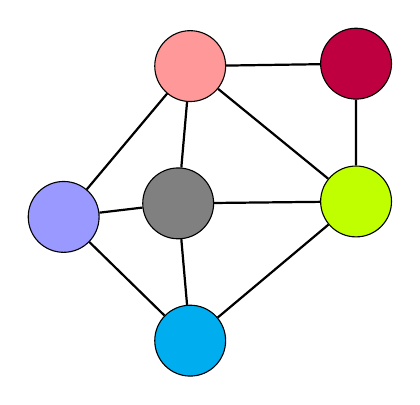
\begin{tikzpicture}[bn/.style={circle,fill,draw,text=white,font=\sffamily,minimum
        size=9mm},every node/.append style={bn}]
         \path node[fill=blue!40] (1) {} -- ++ (50:2.5) node[fill=red!40] (2) {} -- ++(-95:1.75) node[fill=black!50] (3) {}
         -- ++(-85:1.75) node (4)[fill=cyan] {} -- ++(40:2.75) node[fill=lime] (5) {}
         -- ++ (0,1.75) node[fill=purple] (6) {} ;
         \draw[thick] foreach \X [count=\Y] in {2,...,6} {(\Y) -- (\X)}
         (6) -- (2) (2) -- (5) (3) -- (5) (1) -- (4) (1) -- (3);
    \end{tikzpicture}
    
    网络模型 (network model)
    \column{0.475\textwidth}
    \begin{forest}
        forked edges,
        for tree={draw,align=center,edge={-latex}}
        [Root
         [1.1]
         [1.2
          [A
           [A.1]
           [A.2]
          ]
          [1.2.2
           [B.1]
           [B.2]
           [B.3]
          ]
         ]
         [1.3]
        ]
    \end{forest}

    层次模型 (hierarchy model)
\end{columns}
\end{frame}


\begin{frame}[fragile]
    \frametitle{实例与模式}
\begin{itemize}
    \item \alert{模式 (schema)}: 数据库的整体设计 (台湾地区译为「綱要」)
    
    根据数据抽象层次的不同,可以分为物理模式、逻辑模式和子模式。
    \item \alert{实例 (instance)}:特定时刻存储在数据库的信息集合
\end{itemize}
\begin{minted}[bgcolor=LightGray]{java}
Dog dog = new Dog("Duke", 3);
dog = new Dog("Tucker", 5);
\end{minted} 

\end{frame}

\begin{frame}
\section{\textcolor{darkmidnightblue}{5. 数据库语言}}  
\Huge{\faIcon{user}} \Large{\faIcon{arrow-right}} \Huge{\faIcon{database}}
\end{frame}

\begin{frame}
    \frametitle{数据库语言}
    数据库系统提供了:
    
    \begin{itemize}
        \item 数据定义语言(data-definition language): 定义数据库模式
        \item 数据操纵语言 (data-manipulation language): 表达数据库的查询和更新
    \end{itemize}
    \begin{tikzpicture}
        \node[fill=yellow,blur shadow={shadow xshift=-0.5ex},
        text width=25em,anchor=south west,rounded corners]
        {SQL (Structured Query Language) 是目前的主流。它是一种声明式的语言,即关注 What,而不是 How。
        };
    \end{tikzpicture} 
\end{frame}
\begin{frame}[fragile]
    \frametitle{DDL}
\begin{columns}
    \column{0.5\textwidth}
    \includegraphics[width=\textwidth]{table/department} 
    \column{0.5\textwidth}
    \begin{minted}[bgcolor=LightGray]{sql}
CREATE TABLE department (
    dept_name   char (20),
    building   char (15),
    budget  numeric (12,2)
);     
    \end{minted} 
\end{columns}
\end{frame}

\begin{frame}[fragile]
    \frametitle{DML}
    \begin{minted}[bgcolor=LightGray]{sql}
SELECT instructor.name
FROM instructor
WHERE instructor.dept_name = 'History';   
    \end{minted} 
    查询 (query) 是对信息进行检索的语句;DML中涉及信息检索的部分叫\alert{查询语言 (query language)} ,但实践中常把查询语言和数据操纵语言作为同义词出现。
\end{frame}

\begin{frame}
    \section{\textcolor{darkmidnightblue}{6. 数据库系统架构}}  
    一句话,数据库系统非常复杂!
\end{frame}

\begin{frame}
    \begin{center}
        \includegraphics[height=.95\paperheight]{DBMS}
    \end{center}

    

\end{frame}

\begin{frame}
    \frametitle{数据库应用架构}
    \begin{tikzpicture}[
        node distance=2cm,
        title/.style={font=\color{black!50}\ttfamily, fill=orange!30,},
        typetag/.style={rectangle, draw=black!50, font=\ttfamily}
      ]
      
        \node (user1) [typetag, yshift=1.5cm] { 用户 (user) };
        \node (app1) [below=of user1, typetag, yshift=1.5cm,fill=blue!30] { 应用 (application) }; 

        \node (comp1) [title, right=of user1] { \normalsize 客户端};

        \draw[-, thick] (user1) -- (app1);
      
        \node [dashed, draw=black!50,  fit={(user1) (app1)}] (client1){};
      
        \node (db1) [below=of client1, typetag, align=left, fill=blue!30] { 数据库系统 \\(database system) };

        \node (comp2) [title, below=of comp1] { \normalsize 网络};

        \node (comp3) [title, below=of comp2, yshift=1cm] { \normalsize 服务器};

        \node [dashed, draw=black!50,  fit={(db1)}] (server1){};

        \draw[-, thick] (client1) -- (server1);

        \node (user2) [typetag, right=of comp1] { 用户 };
        \node (app2) [below=of user2, typetag, yshift=1.5cm, fill=blue!30] { 应用客户端}; 

        \draw[-, thick] (user2) -- (app2);
      
        \node [dashed, draw=black!50,  fit={(user2) (app2)}] (client2){};

        \node (appserver) [below=of client2, typetag,fill=blue!30, yshift=0.5cm] { 应用服务器};
        \node (db2) [below=of appserver, typetag, fill=blue!30, yshift=1.5cm] { 数据库系统};
        \draw[-, thick] (appserver) -- (db2);
        \node [dashed, draw=black!50,  fit={(appserver) (db2)}] (server2){}; 

        \draw[-, thick] (client2) -- (server2);
      \end{tikzpicture}
\end{frame}
\begin{frame}
    \section{\textcolor{darkmidnightblue}{总结}}   
\begin{enumerate}
    \item 什么是数据库、DBMS?
    \item 为什么要用数据库?
    \item 数据抽象
    \item 数据模型
    \item DDL 和 DML
\end{enumerate}
\end{frame}

\begin{frame}
    \frametitle{《别闹了,费曼先生》}
    \begin{columns}
        \column{0.15\textwidth}
        \includegraphics[height=0.5\paperheight]{image/feynman}
        \column{0.85\textwidth}
        \begin{quote}
            看见那只鸟了吗?那是一只短雉转鸣鸟,但是在德国它被叫作halzenfugel,在中国他被叫作Chung Ling,\alert{即便你知道它所有的名字,你依然对这只鸟一无所知}。你只是对人有一点理解罢了:你知道人们怎么叫这只鸟。现在你看,这只短雉转鸣鸟在歌唱,在教导幼鸟学习飞行,它在夏天横跨整个国家横渡上万英里,但是没有人知道它是如何辨别方向的。\alert{这是一个很简单的道理:知道一件事的名称,并不等同于真正理解它}。
        \end{quote} 
    \end{columns}
    

\end{frame}

\begin{frame}
    \frametitle{本周任务}
\begin{itemize}
    \item 下载并安装飞书,PG 和 DataGrip
    \item 看书了解数据库的发展历史
\end{itemize}   

\pause
\noindent\rule{\textwidth}{1pt}

PostgreSQL:

\begin{itemize}
    \item \faIcon{windows} Windows:从 EDB 下载\href{https://www.enterprisedb.com/downloads/postgres-postgresql-downloads}{安装包}或\href{https://www.enterprisedb.com/download-postgresql-binaries}{二进制包}。
    \item \faIcon{apple} MacOS:从\href{https://postgres.app/}{Postgres.app}下载。
\end{itemize}   

\end{frame}

\end{document}